\chapter{Simplificación Probabilística del Principio de Barlow}
\label{cap:leworldmodel}

A lo largo de los capítulos anteriores hemos asistido a una progresión conceptual: el colapso trivial en las redes siamesas (Capítulo~\ref{cap:siamesas_colapso}) motivó la introducción de fuerzas repulsivas mediante muestras negativas (Capítulo~\ref{cap:contrastive}); la intratabilidad del muestreo negativo en alta dimensión impulsó métodos no contrastivos basados en momentos de segundo orden como Barlow Twins y VICReg (Capítulo~\ref{cap:nocontrastive}), su extensión al caso temporal (Capítulo~\ref{cap:modelos_mundo}) reveló la inestabilidad de las regularizaciones matriciales complejas (PLDM) así como el carácter heurístico de las alternativas arquitectónicas (V-JEPA).

Estos métodos comparten la hipótesis de \textbf{normalidad} de la distribución del espacio de representaciones $\mathcal{Z}$ (que ninguno verifica ni impone). El Puente de Jaynes establece que la decorrelación lineal ($\rho_{kl} = 0$) implica independencia estadística $I(z_k; z_l) = 0$, \emph{si y solo si}, la distribución conjunta es gaussiana. Barlow Twins opera sobre la correlación cruzada $C$; VICReg sobre la covarianza $\Sigma_\mathcal{Z}$; ambos son herramientas de segundo orden que capturan la dependencia lineal, pero son ciegos ante dependencias de orden superior. En la Sección~\ref{sec:conclusiones_barlow} mostramos que, si la distribución de $\mathcal{Z}$ no es gaussiana, dos dimensiones pueden tener covarianza nula y, sin embargo, mantener información mutua no nula.

En este capítulo responderemos a la pregunta: \emph{¿es posible diseñar una regularización que fuerce activamente la normalidad gaussiana de $\mathcal{Z}$, convirtiendo en exacta la aproximación que Barlow Twins y VICReg solo asumían?} La respuesta la ofrece \textbf{SIGReg} propuesta por Balestriero y LeCun (2025)~\cite{balestriero2025lejepa} que combina: el Teorema de Cramér-Wold (1936)~\cite{cramer1936some} (relaciona distribución multivariante con sus respectivas proyecciones univariantes) y el estadístico de Epps-Pulley (1983)~\cite{epps1983test} (test de bondad de ajuste a distribución normal, plenamente diferenciable). El resultado es un \emph{único término} que reemplaza los tres términos de la función de pérdida de VICReg y los siete de PLDM.

\section{Reformulación del Principio de Barlow}
\label{sec:normalidad_barlow}

En los capítulos anteriores, los métodos de aprendizaje de representaciones se han fundamentado en inducir la independencia estadística asumiendo ciegamente la normalidad de los datos para que el Puente de Jaynes sea válido. Esta sección establece una equivalencia que nos libra de esta limitación: forzar directamente que la distribución sea una gaussiana isótropa engloba y resuelve el problema completo, sin tener que regularizar explícitamente la matriz de covarianza ni depender de la suposición de Jaynes.

\begin{definition}[Distribución Normal Isótropa]
\label{def:normal_isotropa}
Sea $Z \in \mathbb{R}^d$ un vector aleatorio continuo. Se dice que $Z$ sigue una distribución \emph{normal isótropa} (o esférica), denotada $Z \sim \mathcal{N}(\vec{0}, I_d)$, si su densidad conjunta es
\begin{equation}
p(z) = \frac{1}{(2\pi)^{d/2}} \exp\left(-\frac{1}{2}\|z\|_2^2\right).
\end{equation}
\end{definition}

\begin{proposition}[Independencia y Principio de Barlow]
\label{prop:normal_barlow}
Si $Z \sim \mathcal{N}(\vec{0}, I_d)$, entonces sus componentes $\{z_1, \dots, z_d\}$ son mutuamente independientes. En el contexto del aprendizaje de representaciones, esto implica que se cumple el Principio de Barlow.
\end{proposition}

\begin{proof}
Como se observa en la densidad conjunta de la Definición~\ref{def:normal_isotropa}, la función exponencial se factoriza analíticamente en el producto de densidades marginales univariantes:
\begin{equation*}
p(z) = \frac{1}{(2\pi)^{d/2}} \exp\left(-\frac{1}{2}\sum_{i=1}^d z_i^2\right) = \prod_{i=1}^d \left( \frac{1}{\sqrt{2\pi}} \exp\left(-\frac{1}{2} z_i^2\right) \right) = \prod_{i=1}^d p(z_i).
\end{equation*}
Esta factorización exacta de la probabilidad conjunta constituye la definición de independencia estadística, logrando por definición el objetivo del Principio de Barlow.
\end{proof}

En particular, $Z$ tiene media nula ($\mathbb{E}[Z]=\vec 0$) y matriz de covarianza identidad ($\Sigma_\mathcal{Z}=I_d$), pero estas dos condiciones por sí solas \textbf{no} caracterizan a la distribución: existen vectores aleatorios con media nula y covarianza $I_d$ que no son gaussianos\footnote{Por ejemplo, $Z=(Z_1,Z_2)$ con $Z_1,Z_2$ i.i.d.\ uniformes en $(-\sqrt3,\sqrt3)$ satisface $\mathbb{E}[Z]=\vec 0$ y $\Sigma_\mathcal{Z}=I_2$, pero su densidad es la indicatriz de un cuadrado, no la de una gaussiana.}. La caracterización completa de $\mathcal{N}(\vec 0, I_d)$ requiere verificar la normalidad directamente sobre la densidad conjunta en $\mathbb{R}^d$ con $d \gg 1$ es computacionalmente intratable: los tests multivariantes de normalidad requieren una densidad de muestras que crece exponencialmente con la dimensión, induciendo la misma limitación que el muestreo de negativos en el Capítulo~\ref{cap:contrastive}. El siguiente resultado mitiga este problema reduciendo la caracterización de $Z$ a la de sus proyecciones unidimensionales.


\begin{theorem}[Teorema de Cramér-Wold]
\label{thm:cramer_wold}
Sean $P$ y $Q$ dos medidas de probabilidad sobre $\mathbb{R}^d$. Si para cada vector unitario $\mathbf{u} \in \mathbb{S}^{d-1}$ (dirección) las proyecciones unidimensionales $P_{\mathbf{u}}$ y $Q_{\mathbf{u}}$ (definidas mediante $z \mapsto \mathbf{u}^T z$) coinciden, entonces $P = Q$~\cite{cramer1936some}.
\end{theorem}

\begin{figure}[H]
\centering
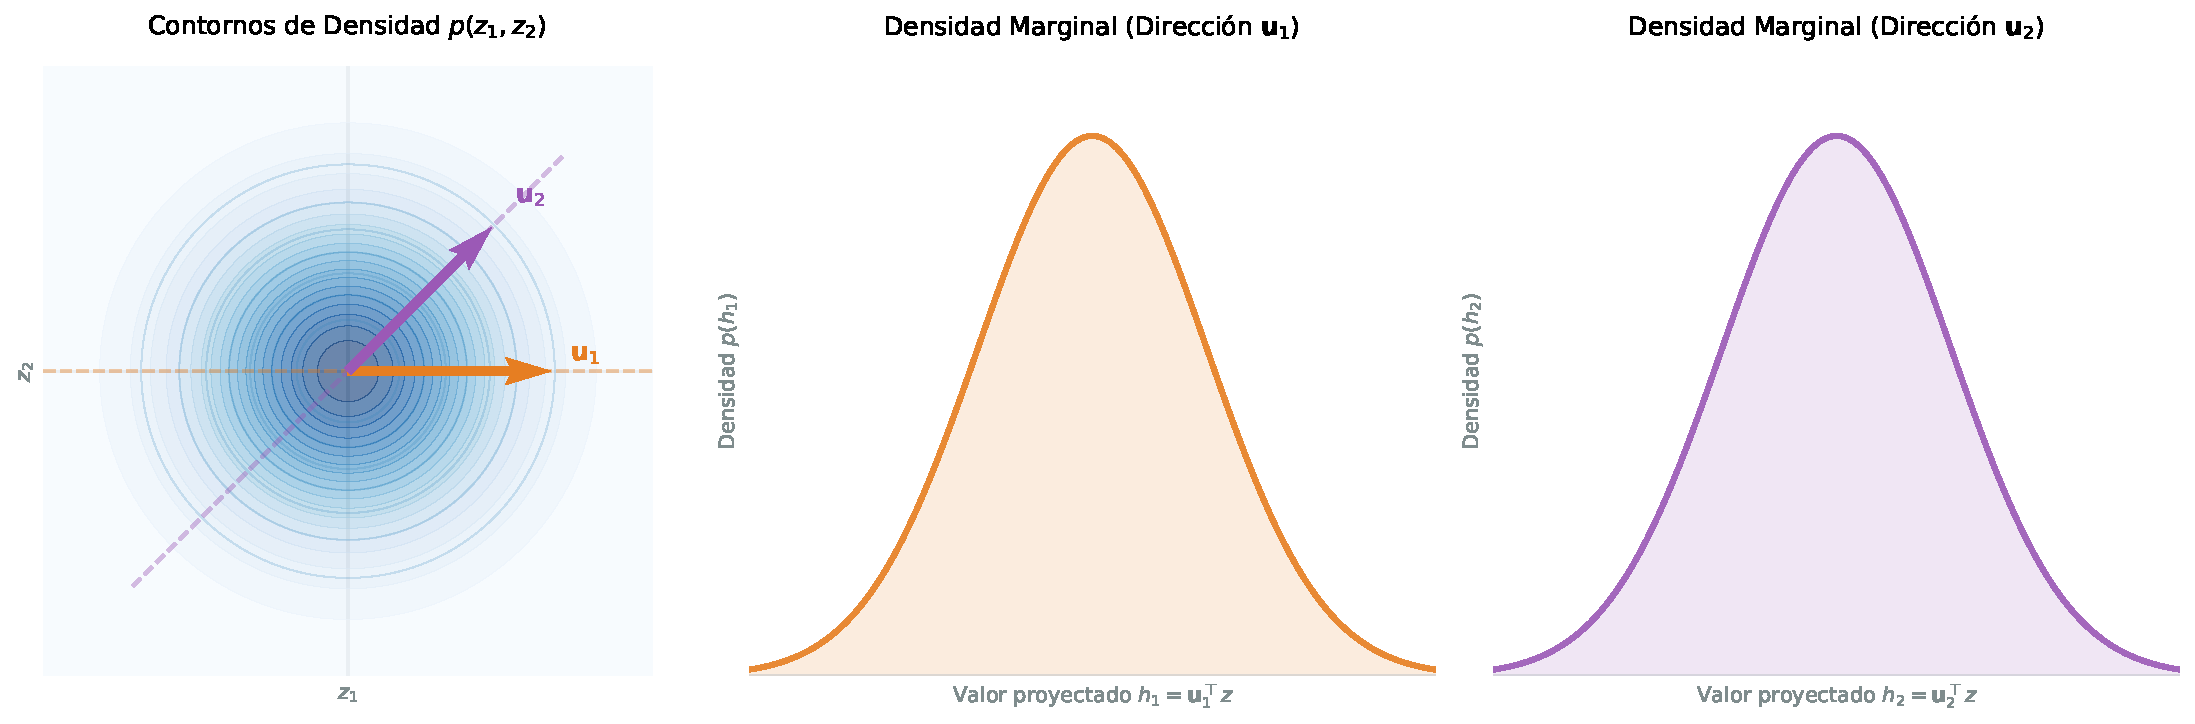
\includegraphics[width=\linewidth]{cramer_wold.pdf}
\caption{Ilustración de la descomposición de Cramér-Wold. \textbf{Izquierda:} Contornos de la densidad en el espacio latente $\mathcal{Z}$, mostrando la descomposición continua a lo largo de dos direcciones unitarias arbitrarias $\mathbf{u}_1$ y $\mathbf{u}_2$. \textbf{Centro:} Densidad marginal proyectada a lo largo de la dirección $\mathbf{u}_1$. \textbf{Derecha:} Densidad marginal proyectada a lo largo de la dirección $\mathbf{u}_2$. El teorema establece que la distribución conjunta queda caracterizada de forma única por el conjunto completo de sus proyecciones unidimensionales.}
\label{fig:cramer_wold_idea}
\end{figure}

\begin{proposition}[Caracterización de la Gaussiana Estándar por Proyecciones]
\label{prop:equivalencia_barlow}
Sea $Z \in \mathbb{R}^d$ un vector aleatorio. Las siguientes afirmaciones son equivalentes:
\begin{enumerate}
    \item[(a)] Para toda dirección $u \in \mathbb{S}^{d-1}$, la proyección $u^\top Z$ sigue una distribución $\mathcal{N}(0,1)$.
    \item[(b)] $Z \sim \mathcal{N}(\vec{0}, I_d)$.
\end{enumerate}
\end{proposition}

\begin{proof}
\textbf{(b $\implies$ a).}
Si $Z \sim \mathcal{N}(\vec 0, I_d)$, toda combinación lineal $u^\top Z$ con $\|u\|=1$ es gaussiana con media $u^\top \vec 0 = 0$ y varianza $u^\top I_d u = \|u\|^2 = 1$. Por tanto $u^\top Z \sim \mathcal{N}(0,1)$ para toda $u\in\mathbb{S}^{d-1}$.

\textbf{(a $\implies$ b).}
Sea $W \sim \mathcal{N}(\vec 0, I_d)$. Por la implicación anterior, $u^\top W \sim \mathcal{N}(0,1)$ para toda $u\in\mathbb{S}^{d-1}$, idéntico a la hipótesis (a) sobre $Z$. Así, $Z$ y $W$ tienen exactamente las mismas leyes de proyección unidimensional. Por el Teorema de Cramér-Wold (Teorema~\ref{thm:cramer_wold}), la ley conjunta de un vector aleatorio en $\mathbb{R}^d$ queda determinada de forma única por el conjunto de sus proyecciones unidimensionales. Por tanto $Z \stackrel{d}{=} W$, es decir, $Z \sim \mathcal{N}(\vec 0, I_d)$.
\end{proof}
Estos resultados suponen pasar de imponer independencia asumiendo normalidad (el Puente de Jaynes), a imponer la normalidad en toda proyección y obtener la independencia como consecuencia. Además reduce el problema de testear normalidad multivariante a la resolución de múltiples tests univariantes en $\mathbb{R}$. Falta aún un test de normalidad que sea diferenciable, es decir, compatible con el descenso de gradiente.

\section{El Test de Epps-Pulley Diferenciable}
\label{sec:epps_pulley}

La Proposición~\ref{prop:equivalencia_barlow} reduce la verificación de la normalidad isótropa de $Z \in \mathbb{R}^d$ a comprobar que cada proyección univariante $u^\top Z$ siga una distribución $\mathcal{N}(0,1)$. Todo el trabajo de esta sección transcurre, por tanto, en $\mathbb{R}$: se busca un test que determine si una variable aleatoria real se distribuye como una normal estándar. Los tests clásicos de normalidad como Shapiro-Wilk, Anderson-Darlingo Kolmogorov-Smirnov, se apoyan en la ordenación de la muestra o en la función de distribución empírica, operaciones que involucran comparaciones y máximos no diferenciables e incompatibles con el descenso de gradiente.

En 2025~\cite{balestriero2025lejepa} se propuso el uso del estadístico de Epps y Pulley~\cite{epps1983test} que, al formular el test de normalidad mediante la \textbf{funcion característica}, cumple con las propiedades de diferenciabilidad buscadas. 

\begin{definition}[Función Característica]
\label{def:funcion_caracteristica}
Sea $X$ una variable aleatoria real distribuida según $P_X$. La función característica de $X$ es la aplicación $\phi_X : \mathbb{R} \to \mathbb{C}$ dada por
\begin{equation}
\phi_X(t) \;=\; \mathbb{E}\!\left[e^{itX}\right] \;=\; \int_{-\infty}^{\infty} e^{itx}\, dP_X(x),
\end{equation}
donde $i = \sqrt{-1}$ es la unidad imaginaria.
\end{definition}

La función característica existe para toda variable aleatoria y su  satisface que: dos variables aleatorias tienen la misma distribución \emph{si y solo si} comparten la misma función característica (\textbf{Teorema de Unicidad}). Esto hace de $\phi_X$ un identificador completo de la distribución. Por tanto, comparar $\phi_X$ con la función característica de $\mathcal{N}(0,1)$ equivale exactamente a testear la normalidad de la distribución $X$.

\begin{proposition}[Función Característica de $\mathcal{N}(0,1)$]
\label{prop:cf_normal}
Si $X \sim \mathcal{N}(0,1)$, su función característica es
\begin{equation}
\phi_0(t) = e^{-t^2/2}.
\label{eq:cf_normal}
\end{equation}
\end{proposition}

\begin{proof}
Se calcula la esperanza de la Definición~\ref{def:funcion_caracteristica}:
\begin{equation*}
\phi_0(t) = \int_{-\infty}^{\infty} e^{itx}\, \frac{1}{\sqrt{2\pi}}\, e^{-x^2/2}\, dx = \frac{1}{\sqrt{2\pi}} \int_{-\infty}^{\infty} \exp\!\left(-\frac{x^2 - 2itx}{2}\right) dx.
\end{equation*}
Completando el cuadrado en el exponente, $x^2 - 2itx = (x - it)^2 + t^2$, se obtiene
\begin{equation*}
\phi_0(t) = e^{-t^2/2}\; \underbrace{\frac{1}{\sqrt{2\pi}} \int_{-\infty}^{\infty} e^{-(x-it)^2/2}\, dx}_{=\, 1} \;=\; e^{-t^2/2},
\end{equation*}
donde la integral compleja vale $1$ por Teorema Integral de Cauchy.
\end{proof}

Cabe destacar que $\phi_0$ resulta ser una función \emph{real y positiva}. Con estas herramientas, la idea del test de Epps-Pulley se formula del siguiente modo: si la variable $X$ siguiera una distribución normal estándar $\mathcal{N}(0,1)$, su función característica $\phi_X$ coincidiría con $\phi_0$ en todo punto $t \in \mathbb{R}$. Por tanto, podemos evaluar esta smilitud usando la distancia $L^2$ entre $\phi_0$ y $\phi_X$:
\begin{equation}
T \;=\; \int_{-\infty}^{\infty} \left|\phi_X(t) - \phi_0(t)\right|^2\, w(t)\, dt,
\label{eq:epps_poblacional}
\end{equation}
donde $w(t) = \sqrt{2}\, e^{-t^2}$ es un peso que concentra la comparación y hace que la integral tenga solución anlítica exacta. $T$ es cero si y solo si $\phi_X = \phi_0$ en casi todo punto, lo que por el Teorema de Unicidad equivale a $X \sim \mathcal{N}(0,1)$.

Nótese que $T$ es un funcional \emph{poblacional}: depende de la distribución verdadera de $X$. En la práctica, solo disponemos de una muestra finita de observaciones $h_1, \dots, h_n$ generadas a partir de $X$. Para testear la normalidad a partir de esta muestra, se estima la función característica poblacional mediante la \textbf{Función Característica Empírica} (FCE):
\begin{equation}
\hat{\phi}_n(t) = \frac{1}{n} \sum_{j=1}^{n} e^{i\, t\, h_j}.
\end{equation}
Al sustituir $\phi_X$ por $\hat{\phi}_n$ en el funcional poblacional~\eqref{eq:epps_poblacional} y resolver la integral ponderada de forma analítica, se obtiene la \textbf{forma cerrada} del estadístico de Epps-Pulley para la muestra:
\begin{equation}
T(h_1, \dots, h_n) = 1 + \frac{\sqrt{2}}{n^2} \sum_{j=1}^{n} \sum_{k=1}^{n} \exp\!\left(-\frac{(h_j - h_k)^2}{4}\right) - \frac{4}{\sqrt{3}\, n} \sum_{j=1}^{n} \exp\!\left(-\frac{h_j^2}{6}\right)
\label{eq:epps_cerrada}
\end{equation}

Se elige este estadístico por su \textbf{diferenciabilidad}. Como se observa en~\eqref{eq:epps_cerrada}, el estadístico es una suma de funciones exponenciales, por tanto, cada término es infinitamente diferenciable con respecto a las observaciones $h_j$. 

Esta propiedad contrasta con los tests clásicos. El estadístico de Kolmogorov-Smirnov, por ejemplo, se define como $D = \sup_t |F_n(t) - \Phi(t)|$, donde $F_n$ es la distribución empírica acumulada y $\sup$ es la operación supremo, que cuenta con discontinuidades y carece de gradientes en dichos puntos, invalidando su uso como función de pérdida para el descenso de gradiente.

\section{El Algoritmo SIGReg y la Pérdida de LeWorldModel}
\label{sec:sigreg_algoritmo}

\subsection{Del Espacio Latente a las Proyecciones Univariantes}
La sección anterior definió el estadístico empírico de Epps-Pulley para una muestra genérica unidimensional. En la práctica, esta muestra proviene de las representaciones producidas por el encoder $f_\theta$, procesadas en batches de $N$ muestras de datos durante cada iteración del optimizador.

En el contexto general del aprendizaje de representaciones, estas muestras pueden provenir de cualquier dominio. Frecuentemente, presentan una dimensión estructural $T$, como secuencias de observaciones (p.e., $T$ instantes de una secuencia de vídeo) o regiones espaciales (como $T$ parches de una imagen), generando un tensor de representaciones en $\mathbb{R}^{N \times T \times d}$. Para aplicar la regularización, este tensor se aplana en una única matriz $Z \in \mathbb{R}^{B \times d}$, con $B = N \cdot T$, que reúne las $B$ representaciones $d$-dimensionales del lote. Cada fila $z_b \in \mathbb{R}^d$ es el embedding de un elemento individual concreto (p.e. un instante específico de una trayectoria en el caso del vídeo).

Para evaluar la normalidad de $Z$ a lo largo \textbf{una dirección} $\mathbf{u} \in \mathbb{S}^{d-1}$, se calcula la proyección univariante de cada embedding:
\begin{equation}
h_b = \mathbf{u}^\top z_b, \quad b = 1, \dots, B,
\end{equation}
obteniendo un vector de $B$ valores reales (número de muestras) $\mathbf{h_u} = (h_1, \dots, h_B)^\top = Z\mathbf{u} \in \mathbb{R}^B$, es decir el lote de observaciones proyectado sobre la dirección $\mathbf{u}$. Según la Proposición~\ref{prop:equivalencia_barlow}, si estas proyecciones se distribuyen como $\mathcal{N}(0,1)$ para todas las direcciones, entonces la distribución multivariante de los datos sigue una normal isótropa $\mathcal{N}(\vec{0}, I_d)$. Dado que el vector $\mathbf{h_u}$ constituye una muestra de tamaño $B$ de la distribución a lo largo de $\mathbf{u}$, su ajuste respecto una normal estándar se puede cuantificar evaluando el estadístico de Epps-Pulley sobre estas observaciones $T(\mathbf{h_u}) = T(h_1, \dots, h_B)$. Repitiendo este proceso para todas las direcciones, se obtiene un test de normalidad multivariante isotrópa. 

\subsection{El Regularizador SIGReg}

\textbf{SIGReg} (\textit{Sketched-Isotropic-Gaussian Regularizer}) combina la reducción dimensional de Cramér-Wold con el test de Epps-Pulley. En cada paso de entrenamiento, se muestrean $M$ direcciones unitarias $\mathbf{u}^{(1)}, \dots, \mathbf{u}^{(M)}$ uniformemente en la esfera $\mathbb{S}^{d-1}$, se calculan las $M$ proyecciones univariantes
\begin{equation}
\mathbf{h}^{(m)} = Z\, \mathbf{u}^{(m)} \in \mathbb{R}^B, \quad m = 1, \dots, M,
\end{equation}
y se promedia el estadístico de Epps-Pulley sobre todas ellas:
\begin{equation}
\text{SIGReg}(Z) = \frac{1}{M} \sum_{m=1}^{M} T\!\left(\mathbf{h}^{(m)}\right).
\end{equation}
Este escalar mide cuánto se desvían las proyecciones de $Z$ respecto a la normalidad. Al minimizarlo, se fuerza a la distribución multivariante a converger hacia $\mathcal{N}(\vec{0}, I_d)$, realizando el Principio de Barlow sin necesidad de regularizar la matriz de covarianza. El resultado es un único término que sustituye simultáneamente los tres términos de VICReg y los siete de PLDM, eliminando los gradientes en conflicto descritos en la Sección~\ref{sec:inestabilidad_gradientes}.

La pérdida total para entrenar LeWorldModel de extremo a extremo es
\begin{equation}
\mathcal{L}_{\text{LeWM}} = \mathcal{L}_{\text{pred}} + \lambda\, \text{SIGReg}(Z),
\end{equation}
con $\mathcal{L}_{\text{pred}} = \frac{1}{NT} \sum_{i=1}^{N} \sum_{t=1}^{T-1} \| \hat{z}_{t+1}^{(i)} - z_{t+1}^{(i)} \|_2^2$ (Capítulo~\ref{cap:modelos_mundo}) y $\lambda > 0$ como único hiperparámetro de regularización.

\begin{figure}[H]
\centering
\resizebox{\linewidth}{!}{
\begin{tikzpicture}[
    node distance=1.5cm,
    inputbox/.style={draw, rectangle, rounded corners, minimum width=2.2cm, minimum height=0.8cm, align=center, fill=gray!5, font=\footnotesize\sffamily},
    matbox/.style={draw, rectangle, rounded corners, minimum width=2.5cm, minimum height=1cm, align=center, fill=gray!5, font=\footnotesize\sffamily},
    termbox/.style={draw, rectangle, rounded corners, minimum width=2.5cm, minimum height=1cm, align=center, font=\footnotesize\bfseries},
    arrow/.style={->, >=stealth, thick, rounded corners},
    operator/.style={draw, circle, fill=gray!10, font=\footnotesize\bfseries, inner sep=2pt}
]

% Inputs
\node[inputbox] (z_hat) at (-5.5, 0) {Predicciones (Batch)\\$\hat{Z} \in \mathbb{R}^{B \times d}$};
\node[inputbox] (z_tgt) at (-2.0, 0) {Objetivos (Batch)\\$Z \in \mathbb{R}^{B \times d}$};
\node[inputbox] (z_all) at (5.5, 0) {Representaciones (Batch)\\$Z \in \mathbb{R}^{B \times d}$};

% Pred Loss
\node[termbox, fill=red!10] (l_pred) at (-3.75, -2.5) {MSE\\{\scriptsize Error cuadrático}};
\draw[arrow] (z_hat) |- (l_pred);
\draw[arrow] (z_tgt) |- (l_pred);

% SIGReg Branch
\node[draw=blue!30, dashed, rounded corners, fill=blue!2, inner sep=10pt, minimum width=8.5cm, minimum height=4.2cm] (cw_box) at (5.5, -3.2) {};
\node[font=\footnotesize\bfseries, text=blue!80] at (3.8, -1.5) {Cramér-Wold (Proyecciones)};

\node[align=left, font=\scriptsize] (u1) at (2.5, -2.4) {$\mathbf{h}^{(1)} = Z \mathbf{u}^{(1)}$};
\node[font=\scriptsize] at (2.5, -3.2) {$\vdots$};
\node[align=left, font=\scriptsize] (uM) at (2.5, -4.0) {$\mathbf{h}^{(M)} = Z \mathbf{u}^{(M)}$};

% Insertar imagen externa en lugar de dibujar con TikZ
\node[inner sep=0pt] at (7.0, -3.2) {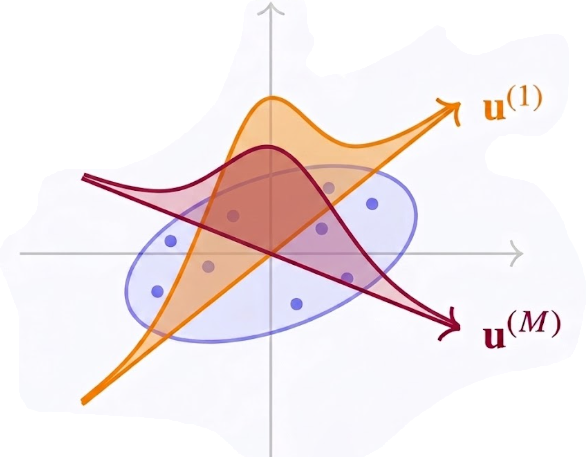
\includegraphics[width=4.5cm]{cramer_wold_new.png}};

\draw[arrow] (z_all) -- (cw_box);

% Epps-Pulley Tests
\node[matbox, fill=orange!10, draw=orange!50] (ep1) at (2.5, -6.5) {Epps-Pulley\\$T(\mathbf{h}^{(1)})$};
\node[matbox, fill=purple!10, draw=purple!50] (epM) at (8.5, -6.5) {Epps-Pulley\\$T(\mathbf{h}^{(M)})$};
\node[font=\footnotesize\bfseries] (dots) at (5.5, -6.5) {$\dots$};

\draw[arrow, orange] (2.5, -5.3) -- (ep1.north);
\draw[arrow, purple] (8.5, -5.3) -- (epM.north);

% Averaging
\node[operator] (avg) at (5.5, -8) {$\frac{1}{M} \sum$};
\draw[arrow, orange] (ep1.south) |- (avg.west);
\draw[arrow, purple] (epM.south) |- (avg.east);

% SIGReg Loss
\node[termbox, fill=blue!10] (l_sigreg) at (5.5, -9.5) {$\text{SIGReg}(Z)$\\{\scriptsize Normalidad}};
\draw[arrow] (avg) -- (l_sigreg);

% Final Total Loss
\node[operator] (plus) at (0.9, -11) {$+$};
\draw[arrow] (l_pred.south) |- (plus.west);
\draw[arrow] (l_sigreg.south) |- (plus.east);
\node[anchor=south west, font=\footnotesize] at (plus.east) {$\times \lambda$};

\node[termbox, fill=green!15, minimum width=4cm] (l_total) at (0.9, -12.5) {$\mathcal{L}_{\text{LeWM}}$\\{\scriptsize $\mathcal{L}_{\text{pred}} + \lambda \text{SIGReg}(Z)$}};
\draw[arrow] (plus) -- (l_total);

% Background Groups
\begin{scope}[on background layer]
    \node[draw=gray, dashed, rounded corners, fit=(l_pred)(z_hat)(z_tgt), inner sep=12pt, fill=gray!3] (pred_bg) {};
    \node[anchor=south, font=\footnotesize\bfseries, text=gray!60] at (pred_bg.north) {$\mathcal{L}_\text{Pred}$};
    
    \node[draw=gray, dashed, rounded corners, fit=(z_all)(cw_box)(ep1)(epM)(l_sigreg), inner sep=15pt, fill=gray!3] (sigreg_bg) {};
    \node[anchor=south, font=\footnotesize\bfseries, text=gray!60] at (sigreg_bg.north) {$\mathcal{L}_\text{SIGReg}$};
\end{scope}

\end{tikzpicture}
}
\caption{Esquema detallado de la función de pérdida de LeWorldModel. A la izquierda, la rama de predicción optimiza la similitud en el espacio latente (p.e. minimizando el error cuadrático medio). A la derecha, la rama de regularización aplica SIGReg al conjunto de representaciones del batch. Nótese que el lote de representaciones $Z \in \mathbb{R}^{B \times d}$ de la rama derecha (regularización) coincide exactamente con los objetivos reales $Z \in \mathbb{R}^{B \times d}$ de la rama izquierda (predicción): mediante Cramér-Wold se proyectan los datos multivariantes sobre múltiples direcciones aleatorias $\mathbf{u}^{(m)}$, a continuación se evalúa el ajuste a una normal univariante con el estadístico de Epps-Pulley $T$ para cada proyección, y se promedian los resultados. Ambos términos se combinan ponderados por $\lambda$.}
\label{fig:lewm_loss_schema}
\end{figure}

\begin{figure}[H]
\centering
\resizebox{\linewidth}{!}{
\begin{tikzpicture}[
    node distance=1.5cm,
    obsbox/.style={draw=gray!50, rectangle, rounded corners, minimum width=2cm, minimum height=1cm, align=center, fill=gray!5, font=\footnotesize\sffamily},
    encbox/.style={draw=blue!40, rectangle, rounded corners, minimum width=2cm, minimum height=1cm, align=center, fill=blue!5, font=\footnotesize\sffamily},
    predbox/.style={draw=violet!40, rectangle, rounded corners, minimum width=2.2cm, minimum height=1cm, align=center, fill=violet!5, font=\footnotesize\sffamily},
    lossbox/.style={draw=red!40, rectangle, rounded corners, minimum width=2.5cm, minimum height=1.2cm, align=center, fill=red!10, font=\footnotesize\bfseries},
    arrow/.style={->, >=stealth, thick, rounded corners},
    state/.style={font=\footnotesize\sffamily, align=center}
]

    % ===== FILA SUPERIOR (PASO t) =====
    \node[obsbox] (ot) at (0, 0) {Observación\\$o_t$};
    \node[encbox] (enc_t) at (2.8, 0) {Encoder\\$f_\theta$};
    \node[state] (zt) at (5.0, 0) {Estado\\$z_t$};
    \node[predbox] (pred) at (7.8, 0) {Predictor\\$g_\phi$};
    \node[state] (zhat) at (10.4, 0) {Predicción\\$\hat{z}_{t+1}$};

    % ===== FILA INFERIOR (PASO t+1) =====
    \node[obsbox] (ot1) at (0, -2.2) {Observación\\$o_{t+1}$};
    \node[encbox] (enc_t1) at (2.8, -2.2) {Encoder\\$f_\theta$};
    \node[state] (zt1) at (10.4, -2.2) {Objetivo\\$z_{t+1}$};

    % ===== CONEXIONES =====
    \draw[arrow] (ot) -- (enc_t);
    \draw[arrow] (enc_t) -- (zt);
    \draw[arrow] (zt) -- (pred);
    \draw[arrow] (pred) -- (zhat);

    \draw[arrow] (ot1) -- (enc_t1);
    \draw[arrow] (enc_t1) -- (zt1);

    % Pérdida predictiva
    \node[lossbox] (loss_asym) at (13.5, -1.1) {$\mathcal{L}_{\text{LeWM}}$};
    \draw[arrow] (zhat.east) to[out=0, in=180] (loss_asym.west);
    \draw[arrow] (zt1.east) to[out=0, in=180] (loss_asym.west);

    % Pesos compartidos
    \draw[<->, dashed, thick, gray!70] (enc_t.south) -- node[right, font=\scriptsize, text=gray!80] {pesos compartidos} (enc_t1.north);

    % Background Groups
    \begin{scope}[on background layer]
        \node[draw=orange!30, dashed, rounded corners=8pt, fit=(zt) (zhat) (pred), inner sep=10pt, fill=orange!3] (pred_zone) {};
        \node[anchor=south, font=\scriptsize\bfseries, text=orange!80] at (pred_zone.north) {Dinámica latente};
    \end{scope}

\end{tikzpicture}
}
\caption{Arquitectura base de Joint Embedding Predictiva (JEPA) utilizada en LeWorldModel. Un encoder $f_\theta$ (con pesos compartidos) extrae representaciones abstractas de las observaciones, mientras que un predictor $g_\phi$ simula la transición dinámica en el espacio latente anticipando $\hat{z}_{t+1}$ a partir del estado actual $z_t$. Posteriormente, a este modelo se le añadirá la regularización de normalidad isótropa SIGReg detallada a continuación.}
\label{fig:lewm_jepa_arch}
\end{figure}


\section{El Cierre del Círculo de Barlow}
\label{sec:conclusiones_leworldmodel}

Este capítulo culmina el recorrido evolutivo del aprendizaje de representaciones en el paradigma de Joint Embedding, resolviendo la principal limitación teórica de los métodos no contrastivos analizados en el Capítulo~\ref{cap:nocontrastive}.

El principio de reducción de redundancia de Barlow~\cite{barlow1961possible} exige la independencia estadística mutua entre las variables latentes. Bajo el marco clásico de Barlow Twins y VICReg, esta condición se aproximaba mediante la anulación de las covarianzas lineales (momentos de segundo orden), una simplificación que el Puente de Jaynes solo declara exacta bajo una hipótesis de normalidad multivariante que dichos métodos no garantizaban activamente.

A través del regularizador SIGReg se cierra de forma definitiva esta brecha:
\begin{itemize}
    \item \textbf{Fundamento en Cramér-Wold:} Permite proyectar el espacio latente de alta dimensión a múltiples direcciones unidimensionales aleatorias, reduciendo un problema multivariante intratable a una familia de evaluaciones univariantes en paralelo.
    \item \textbf{Diferenciabilidad con Epps-Pulley:} Evalúa la normalidad de cada proyección en el espacio de funciones características de manera analítica y plenamente diferenciable, forzando a la distribución latente a converger de forma suave hacia una Gaussiana isótropa.
\end{itemize}

Al asegurar de manera activa la normalidad esférica de las representaciones, la decorrelación lineal y la independencia estadística se vuelven equivalentes. De este modo, SIGReg no solo simplifica la complejidad computacional y elimina los gradientes en conflicto de VICReg, sino que aplica el principio de Barlow en su pureza matemática original.

La Figura~\ref{fig:arco_narrativo} sintetiza el flujo conceptual completo que vertebra los Capítulos~\ref{cap:siamesas_colapso}--\ref{cap:leworldmodel}.


\begin{figure}[H]
\centering
\resizebox{\linewidth}{!}{%
\begin{tikzpicture}[
    node distance=0.5cm,
    problem/.style={draw=red!70!black, rounded corners, minimum width=2cm, minimum height=1.2cm, align=center, fill=red!8, font=\scriptsize, text=black},
    solution/.style={draw=blue!70!black, rounded corners, minimum width=2cm, minimum height=1.2cm, align=center, fill=blue!8, font=\scriptsize, text=black},
    assumption/.style={draw=yellow!70!black, rounded corners, minimum width=2cm, minimum height=1.2cm, align=center, fill=yellow!10, font=\scriptsize, text=black},
    final/.style={draw=green!60!black, rounded corners, minimum width=2cm, minimum height=1.2cm, align=center, fill=green!10, font=\scriptsize, thick, text=black},
    arrow/.style={->, >=stealth, thick, gray!70},
    label/.style={font=\tiny, text=black, align=center}
]

% Nodos
\node[problem] (collapse) {Colapso\\Trivial y\\Dimensional};
\node[label, above=0.1cm of collapse] {Cap.~3\\(1993)};

\node[solution, right=of collapse] (contrastive) {P\'{e}rdidas\\Contrastivas\\$\mathcal{L}_{\text{neg}}$};
\node[label, above=0.1cm of contrastive] {Cap.~4\\(2006)};

\node[problem, right=of contrastive] (exp) {Escala\\exponencial\\$\mathcal{O}(e^d)$};

\node[solution, right=of exp] (barlow) {Barlow Twins\\VICReg\\(decorrelaci\'{o}n)};
\node[label, above=0.1cm of barlow] {Cap.~5\\(2021--2022)};

\node[assumption, right=of barlow] (gauss) {Hip\'{o}tesis\\Gaussiana\\no verificada};

\node[solution, right=of gauss] (jepa) {V-JEPA\\(heur\'{i}sticas\\ad-hoc)};
\node[label, above=0.1cm of jepa] {Cap.~6\\(2022--2025)};

\node[final, right=of jepa] (sigreg) {\textbf{SIGReg}\\Normalidad\\forzada};
\node[label, above=0.1cm of sigreg] {Cap.~7\\(2025--2026)};

% Flechas
\draw[arrow] (collapse) -- (contrastive);
\draw[arrow] (contrastive) -- (exp);
\draw[arrow] (exp) -- (barlow);
\draw[arrow] (barlow) -- (gauss);
\draw[arrow] (gauss) -- (jepa);
\draw[arrow] (jepa) -- (sigreg);

% Arco de cierre
\draw[->, >=stealth, thick, green!50!black, dashed] (sigreg.south) to[out=-90, in=-90, looseness=0.5] node[below, font=\scriptsize\itshape, text=green!50!black, yshift=-0.1cm] {Cierre del Principio de Barlow} (barlow.south);

% Leyenda
\node[below=1.8cm of collapse, font=\scriptsize, anchor=west] (leg) {
    {\tikz\draw[fill=red!8, draw=red!70!black, rounded corners] (0,0) rectangle (0.4,0.25);} Problema \quad
    {\tikz\draw[fill=blue!8, draw=blue!70!black, rounded corners] (0,0) rectangle (0.4,0.25);} Soluci\'{o}n \quad
    {\tikz\draw[fill=yellow!10, draw=yellow!70!black, rounded corners] (0,0) rectangle (0.4,0.25);} Hip\'{o}tesis pendiente \quad
    {\tikz\draw[fill=green!10, draw=green!60!black, rounded corners] (0,0) rectangle (0.4,0.25);} Resoluci\'{o}n final
};

\end{tikzpicture}%
}
\caption{Arco narrativo evolutivo de los Capítulos~\ref{cap:siamesas_colapso}--\ref{cap:leworldmodel}. Cada limitación (en rojo) motiva la solución siguiente (en azul). La hipótesis gaussiana (en amarillo), asumida implícitamente por Barlow Twins y VICReg pero nunca verificada, es finalmente impuesta de forma explícita por SIGReg (en verde), cerrando el principio de Barlow en su pureza matemática original.}
\label{fig:arco_narrativo}
\end{figure}


\section{Limitaciones, Conclusiones Generales y Líneas Futuras}
\label{sec:conclusiones_generales}

\subsection{Limitaciones del Marco SIGReg/LeWorldModel}
\label{subsec:limitaciones_sigreg}

El marco desarrollado en este capítulo resuelve la tensión planteada en la Sección~\ref{sec:limitaciones_vjepa_pldm}, pero no está libre de supuestos propios que conviene señalar con el mismo rigor con el que se han señalado los de PLDM y V-JEPA.

La primera limitación es que SIGReg fuerza la normalidad de $Z$ mediante un test estadístico diferenciable, pero la elección de la distribución objetivo, la gaussiana isótropa, no es arbitraria, sino que responde a una necesidad técnica; es la única distribución bajo la cual el Puente de Jaynes garantiza la equivalencia entre covarianza nula e independencia. Esto significa que el marco no demuestra que la normalidad sea la estructura óptima del espacio para cualquier tarea, sino que es la estructura que permite cerrar la brecha teórica identificada en la Sección~\ref{sec:barlow_hipotesis}. Si el mundo subyacente que se intenta modelar no admite una representación latente gaussiana sin pérdida de información relevante, imponer esta restricción podría limitar la expresividad de $\mathcal{Z}$.

El análisis del Puente de Jaynes desarrollado en los capítulos precedentes conduce, de forma natural, a una pregunta fundamental: ¿es la gaussianidad únicamente una propiedad que nos permite asegurar que las variables aprendidas sean estadísticamente independientes, o es además la distribución idónea para garantizar que el modelo aprenda las variables reales que describen el entorno? Esta cuestión fue resuelta recientemente por Klindt, LeCun y Balestriero, quienes demostraron formalmente que, bajo una dinámica con ruido aditivo, la distribución gaussiana es la única que permite al modelo recuperar de forma lineal las variables latentes verdaderas del sistema~\cite{klindt2026lejepa}. De este modo, la normalidad que SIGReg impone sobre $\mathcal{Z}$ no es solo una elección conveniente para justificar la independencia matemática, sino la única opción que asegura una correspondencia directa entre la representación aprendida y el estado real del mundo en esta familia de modelos. Por el contrario, si las variables reales del entorno no siguen una distribución gaussiana, este tipo de regularizadores pierde dicha garantía de recuperación, lo que sugiere que para modelar dinámicas no gaussianas se requerirían modificaciones en la arquitectura del modelo y no solo un ajuste de sus hiperparámetros~\cite{klindt2026lejepa}. Este último resultado ~\cite{klindt2026lejepa} publicado a finales de mayo de 2026 resalta cómo el problema que abordamos en el presente trabajo, se encuentra en la frontera activa de la investigación actual, habiendo evolucionado teóricamente de forma paralela a la redacción del mismo.

La segunda limitación es de naturaleza práctica. El test de Epps-Pulley diferenciable introducido en la Sección~\ref{sec:epps_pulley} evalúa la normalidad mediante proyecciones aleatorias en una dimensión, apoyándose en el Teorema de Cramér-Wold (Sección~\ref{sec:cramer_wold}). El número de proyecciones necesarias para que esta aproximación sea fiel a la normalidad multivariada completa crece con la dimensión de $\mathcal{Z}$, lo que introduce un coste computacional adicional respecto a los términos de varianza y covarianza de VICReg, que se calculan de forma cerrada.
